%!TEX TS-program = xelatex
\documentclass[12pt, a4paper]{article}

\usepackage{amsmath,amsfonts,amssymb,amsthm,mathtools} 
\usepackage{fontspec}            % пакет для подгрузки шрифтов
\setmainfont{Amiri}   % задаёт основной шрифт документа

% why do we need \newfontfamily:
% http://tex.stackexchange.com/questions/91507/
\newfontfamily{\cyrillicfonttt}{Amiri}
\newfontfamily{\cyrillicfont}{Amiri}
\newfontfamily{\cyrillicfontsf}{Amiri}
% Иногда тех не видит структуры шрифтов. Эти трое бравых парней спасают ситуацию и доопределяют те куски, которые Тех не увидел.

\usepackage{unicode-math}     % пакет для установки математического шрифта
\setmathfont{Asana Math}      % шрифт для математики

\usepackage{polyglossia}      % Пакет, который позволяет подгружать русские буквы
\setdefaultlanguage{russian}  % Основной язык документа
\setotherlanguage{english}    % Второстепенный язык документа

\usepackage[paper=a4paper,top=2mm, bottom=2mm,left=4mm,right=4mm,includefoot]{geometry}

\usepackage{pgf,tikz,pgfplots}
\usetikzlibrary{arrows,calc}
\usepackage{relsize} 

\usepackage{graphicx} 
\usepackage{graphics}
\graphicspath{{elections/}{elections_pdf/}}

\usepackage{rotating}
\usepackage{xcolor}
\usepackage{color}

\newcommand{\BBig}{\fontsize{60}{60}\selectfont}

\definecolor{bl}{HTML}{333333}
\definecolor{latxlatx}{HTML}{434545}

% Можно, конечно, сделать через foreach, но мне тааак влом...

\newcommand{\nacley}[1]{
\begin{tikzpicture}[scale=1]
            
\node[inner sep=0pt] (russell) at (-2.5,4.4) {\includegraphics[height=5.08cm,width=4.39cm]{#1}};

\node[inner sep=0pt] (russell) at (2.5,4.4) {\includegraphics[height=5.08cm,keepaspectratio]{#1}};                

\node[inner sep=0pt] (russell) at (-7.5,4.4) {\includegraphics[height=5.08cm,width=4.39cm]{#1}}; 

\node[inner sep=0pt] (russell) at (7.5,4.4) {\includegraphics[height=5.08cm,width=4.39cm]{#1}}; 


\node[inner sep=0pt] (russell) at (0,0.4) {\includegraphics[height=5.08cm,width=4.39cm]{#1}};                             

\node[inner sep=0pt] (russell) at (-5,0.4)   {\includegraphics[height=5.08cm,width=4.39cm]{#1}};  

\node[inner sep=0pt] (russell) at (5,0.4) {\includegraphics[height=5.08cm,width=4.39cm]{#1}};   


\node[inner sep=0pt] (russell) at (2.5,-3.6) {\includegraphics[height=5.08cm,width=4.39cm]{#1}}; 
   
\node[inner sep=0pt] (russell) at (-2.5,-3.6) {\includegraphics[height=5.08cm,width=4.39cm]{#1}}; 

\node[inner sep=0pt] (russell) at (-7.5,-3.6) {\includegraphics[height=5.08cm,width=4.39cm]{#1}}; 

\node[inner sep=0pt] (russell) at (7.5,-3.6) {\includegraphics[height=5.08cm,width=4.39cm]{#1}}; 


      
\node[inner sep=0pt] (russell) at (0,-7.6) {\includegraphics[height=5.08cm,keepaspectratio]{#1}};       

\node[inner sep=0pt] (russell) at (5,-7.6) {\includegraphics[height=5.08cm,keepaspectratio]{#1}};  

\node[inner sep=0pt] (russell) at (-5,-7.6) {\includegraphics[height=5.08cm,keepaspectratio]{#1}};  



\node[inner sep=0pt] (russell) at (-2.5,-11.6) {\includegraphics[height=5.08cm,width=4.39cm]{#1}};

\node[inner sep=0pt] (russell) at (2.5,-11.6) {\includegraphics[height=5.08cm,keepaspectratio]{#1}};                

\node[inner sep=0pt] (russell) at (-7.5,-11.6) {\includegraphics[height=5.08cm,width=4.39cm]{#1}}; 

\node[inner sep=0pt] (russell) at (7.5,-11.6) {\includegraphics[height=5.08cm,width=4.39cm]{#1}}; 



\node[inner sep=0pt] (russell) at (0,-15.6) {\includegraphics[height=5.08cm,keepaspectratio]{#1}};       

\node[inner sep=0pt] (russell) at (5,-15.6) {\includegraphics[height=5.08cm,keepaspectratio]{#1}};  

\node[inner sep=0pt] (russell) at (-5,-15.6) {\includegraphics[height=5.08cm,keepaspectratio]{#1}};  



\node[inner sep=0pt] (russell) at (-2.5,-19.6) {\includegraphics[height=5.08cm,width=4.39cm]{#1}};

\node[inner sep=0pt] (russell) at (2.5,-19.6) {\includegraphics[height=5.08cm,keepaspectratio]{#1}};                

\node[inner sep=0pt] (russell) at (-7.5,-19.6) {\includegraphics[height=5.08cm,width=4.39cm]{#1}}; 

\node[inner sep=0pt] (russell) at (7.5,-19.6) {\includegraphics[height=5.08cm,width=4.39cm]{#1}}; 
\end{tikzpicture}
}

\begin{document}

\pagestyle{empty}
\centering

\begin{tikzpicture}[scale=1]

\node[inner sep=0pt] (russell) at (-7.5,4.4) {
\includegraphics[height=5.08cm,width=4.39cm]{nakleyka_Kamila.pdf}}; 
            
\node[inner sep=0pt] (russell) at (-2.5,4.4) {
\includegraphics[height=5.08cm,width=4.39cm]{norm_Liza1.png}};

\node[inner sep=0pt] (russell) at (2.5,4.4) {
\includegraphics[height=5.08cm,keepaspectratio]{norm_Liza1.png}};                


\node[inner sep=0pt] (russell) at (7.5,4.4) {
\includegraphics[height=5.08cm,width=4.39cm]{norm_Liza1.png}}; 


\node[inner sep=0pt] (russell) at (0,0.4) {
\includegraphics[height=5.08cm,width=4.39cm]{b+greater.pdf}};                             


\node[inner sep=0pt] (russell) at (-5,0.4)   {
\includegraphics[height=5.08cm,width=4.39cm]{b+greater.pdf}};  

\node[inner sep=0pt] (russell) at (5,0.4) {
\includegraphics[height=5.08cm,width=4.39cm]{b+greater.pdf}};   


\node[inner sep=0pt] (russell) at (2.5,-3.6) {
\includegraphics[height=5.08cm,width=4.39cm]{beta.pdf}}; 
   
\node[inner sep=0pt] (russell) at (-2.5,-3.6) {
\includegraphics[height=5.08cm,width=4.39cm]{beta-hat.pdf}}; 

\node[inner sep=0pt] (russell) at (-7.5,-3.6) {
\includegraphics[height=5.08cm,width=4.39cm]{beta-hat.pdf}}; 

\node[inner sep=0pt] (russell) at (7.5,-3.6) {
\includegraphics[height=5.08cm,width=4.39cm]{pot.pdf}}; 


      
\node[inner sep=0pt] (russell) at (0,-7.6) {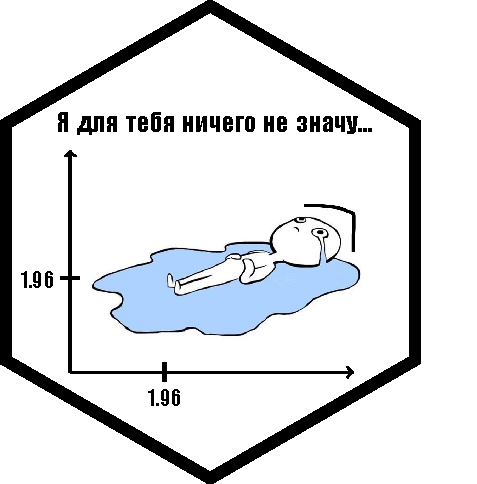
\includegraphics[height=5.08cm,keepaspectratio]{elips.pdf}};       

\node[inner sep=0pt] (russell) at (5,-7.6) {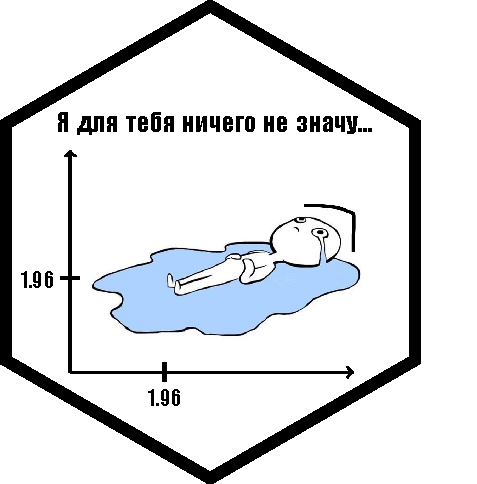
\includegraphics[height=5.08cm,keepaspectratio]{elips.pdf}};  

\node[inner sep=0pt] (russell) at (-5,-7.6) {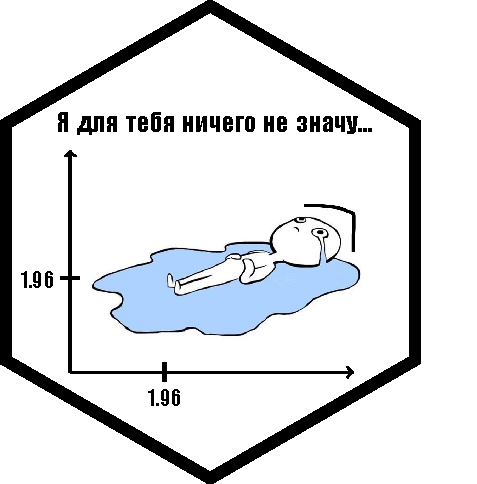
\includegraphics[height=5.08cm,keepaspectratio]{elips.pdf}};  



\node[inner sep=0pt] (russell) at (-2.5,-11.6) {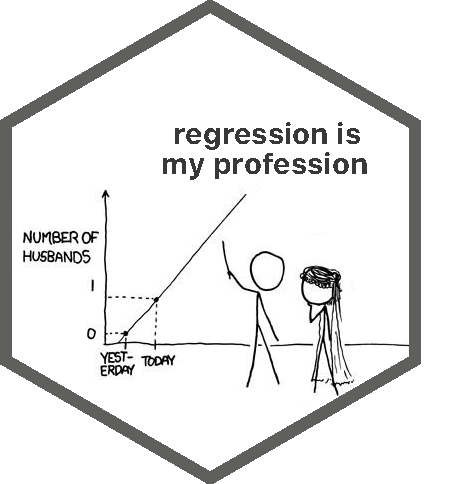
\includegraphics[height=5.08cm,keepaspectratio]{regression_is_my.pdf}};

\node[inner sep=0pt] (russell) at (2.5,-11.6) {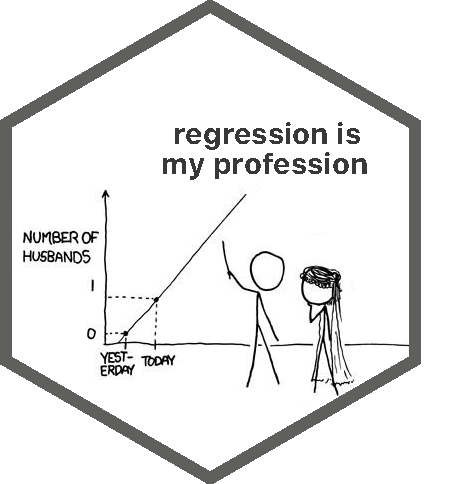
\includegraphics[height=5.08cm,keepaspectratio]{regression_is_my.pdf}};                

\node[inner sep=0pt] (russell) at (-7.5,-11.6) {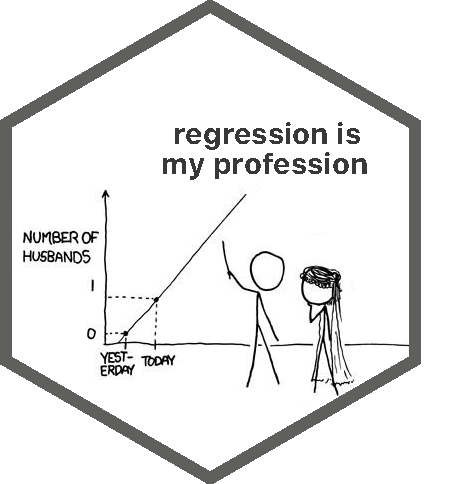
\includegraphics[height=5.08cm,keepaspectratio]{regression_is_my.pdf}}; 

\node[inner sep=0pt] (russell) at (7.5,-11.6) {
\includegraphics[height=5.08cm,keepaspectratio]{LaTeX-sex.pdf}}; 



\node[inner sep=0pt] (russell) at (0,-15.6) {
\includegraphics[height=5.08cm,keepaspectratio]{Bayes.png}};       

\node[inner sep=0pt] (russell) at (5,-15.6) {
\includegraphics[height=5.08cm,keepaspectratio]{Bayes.png}};  

\node[inner sep=0pt] (russell) at (-5,-15.6) {
\includegraphics[height=5.08cm,keepaspectratio]{Bayes.png}};  



\node[inner sep=0pt] (russell) at (-2.5,-19.6) {
\includegraphics[height=5.08cm,width=4.39cm]{zen.pdf}};

\node[inner sep=0pt] (russell) at (2.5,-19.6) {
\includegraphics[height=5.08cm,keepaspectratio]{dummy_trap.pdf}};                

\node[inner sep=0pt] (russell) at (-7.5,-19.6) {
\includegraphics[height=5.08cm,width=4.39cm]{zen.pdf}}; 

\node[inner sep=0pt] (russell) at (7.5,-19.6) {
\includegraphics[height=5.08cm,width=4.39cm]{dummy_trap.pdf}}; 
\end{tikzpicture}



\end{document}
